\documentclass[12pt, a4paper]{article}

% Required Packages
\usepackage[utf8]{inputenc}
\usepackage{geometry}
\geometry{top=2.5cm, bottom=2.5cm, left=2.5cm, right=2.5cm}
\usepackage{booktabs} % For professional looking tables
\usepackage{graphicx} % For inserting images
\usepackage{tabularx} % For tables with automatic line breaks
\usepackage{float}    % For figure placement [H]
\usepackage{amsmath}  % For math formulas
\usepackage{hyperref} % For clickable links and references
\usepackage{setspace} % For line spacing
\setstretch{1.15}

\title{\textbf{Problem 4}}
\author{\textit{[Your Name / Group Name]}}
\date{\today}

\begin{document}

\maketitle

\section{Benchmarks}
To verify the performance and robustness of the Proposed Heuristic, this experiment selected the following two benchmarks for comparison:

\begin{enumerate}
    \item \textbf{Optimal Solution:} By limiting the instance size to a computationally tractable range, we use a mathematical programming solver to solve the problem. This provides the true optimal objective value as an absolute performance baseline.
    \item \textbf{Pure Greedy Algorithm:} Served as a simple and intuitive baseline. The steps of this algorithm are as follows:
    \begin{itemize}
        \item \textbf{Step 1:} Sort all orders in descending order based on "Absolute Revenue". If the revenue is identical, prioritize the order with an earlier pickup time.
        \item \textbf{Step 2:} Iterate through the sorted orders. For each order, search outward from the pickup station (in increasing order of relocation time).
        \item \textbf{Step 3:} Find the nearest available vehicle that satisfies the level and time window constraints. If found, and the remaining relocation budget allows, assign it immediately and deduct the corresponding budget and vehicle availability time; if no vehicle is available, reject the order and evaluate the next one.
    \end{itemize}
\end{enumerate}

\section{Experimental Design}
To comprehensively evaluate the algorithm's performance under various business scenarios, we designed stress tests covering spatial, temporal, and resource dimensions, categorizing them into 7 distinct scenarios.

\subsection{Fixed Parameters}
Across all scenarios, the base environment settings are as follows:
\begin{itemize}
    \item Number of Stations ($|S|$): 20
    \item Number of Cars ($|C|$): 100
    \item Number of Car Levels ($|L|$): 3 (Hourly Rates: Level 1 = 400, Level 2 = 800, Level 3 = 1200)
    \item Total Number of Orders ($|K|$): 200
    \item Planning Horizon ($D$): 7 
    \item Relocation Budget ($B$): 6000
\end{itemize}

\subsection{Test Scenarios and Factors}
By adjusting factors such as order distribution, relocation budget, and fleet structure, we established the following 7 test scenarios. $100$ random instances were generated for each scenario. Note that any parameter not explicitly mentioned in Scenarios 02--07 follows the baseline settings of Scenario 01 unless otherwise specified.

\begin{table}[H]
    \centering
    \caption{Description of Experimental Scenarios}
    \label{tab:scenarios}
    \small
    \begin{tabularx}{\textwidth}{@{}l X@{}}
        \toprule
        \textbf{Scenario} & \textbf{Description \& Parameter Distribution} \\
        \midrule
        01 & Order time, duration, stations, and levels are uniformly distributed. \\
        \addlinespace
        02 & 80\% of orders request Level 1, but the initial fleet consists mostly of high-level cars (L1: 10\%, L2: 40\%, L3: 50\%). \\
        \addlinespace
        03 & From day 1 to day 3, 70\% of the total orders are bad orders (fixed at Level 1) requiring long vehicle occupation (24--48 hrs). From day 4 to day 7, 30\% of the total orders are good orders (fixed at Level 3) requiring short vehicle occupation (4--12 hrs). \\
        \addlinespace
        04 & 80\% of orders originate at stations 1 or 2, but return at the last two stations. \\
        \addlinespace
        05 & Order occurrences are uniform, but orders in the last 2 days have extremely long durations (24--48 hrs); the first 5 days have short durations (2--6 hrs). \\
        \addlinespace
        06 & The first 5 days contain only 30\% of total orders, while the remaining 70\% erupt in the last 2 days; duration remains random. \\
        \addlinespace
        07 & The relocation budget is severely restricted to $B = 2000$ (compared to the baseline $B = 6000$). \\
        \bottomrule
    \end{tabularx}
\end{table}

\section{Results and Analysis}
This section presents the Optimality Gap of the Proposed Heuristic and the Pure Greedy Algorithm relative to the Optimal Solution. The Gap is calculated as:
\begin{equation}
    Gap = \frac{\text{Optimal} - \text{Heuristic}}{\text{Optimal}} \times 100\%
\end{equation}

\subsection{Average Performance and Standard Deviation}
Table \ref{tab:gap_statistics} summarizes the average gaps and standard deviations under each scenario.

\begin{table}[H]
\centering
\caption{Statistics of Optimality Gaps and Standard Deviations by Scenario}
\label{tab:gap_statistics}
\begin{tabular}{lcccc}
\toprule
Group Name (Scenario) & Avg Gap\_H & Std Dev H & Avg Gap\_G & Std Dev G \\
\midrule
01\_All\_Random         & 0.01 \% & 0.09 \% &  6.98 \% &  5.87 \% \\
02\_Upgrade\_Test       & 2.56 \% & 3.85 \% & 36.04 \% & 11.57 \% \\
03\_Value\_Trap         & 4.19 \% & 3.14 \% & 53.46 \% &  7.62 \% \\
04\_Spatial\_Imbalance  & 6.93 \% & 6.67 \% & 11.68 \% &  6.79 \% \\
05\_Late\_Duration\_Peak& 0.00 \% & 0.00 \% &  9.87 \% &  6.10 \% \\
06\_Late\_Quantity\_Peak& 0.68 \% & 1.27 \% &  4.70 \% &  3.67 \% \\
07\_Budget\_Trap        & 5.80 \% & 8.64 \% & 15.69 \% &  7.41 \% \\
\bottomrule
\end{tabular}
\end{table}

\subsection{Performance Visualization}
Figure \ref{fig:performance_chart} illustrates the performance comparison across all scenarios.

\begin{figure}[H]
    \centering
    % Ensure the image file is in the same directory as this .tex file
    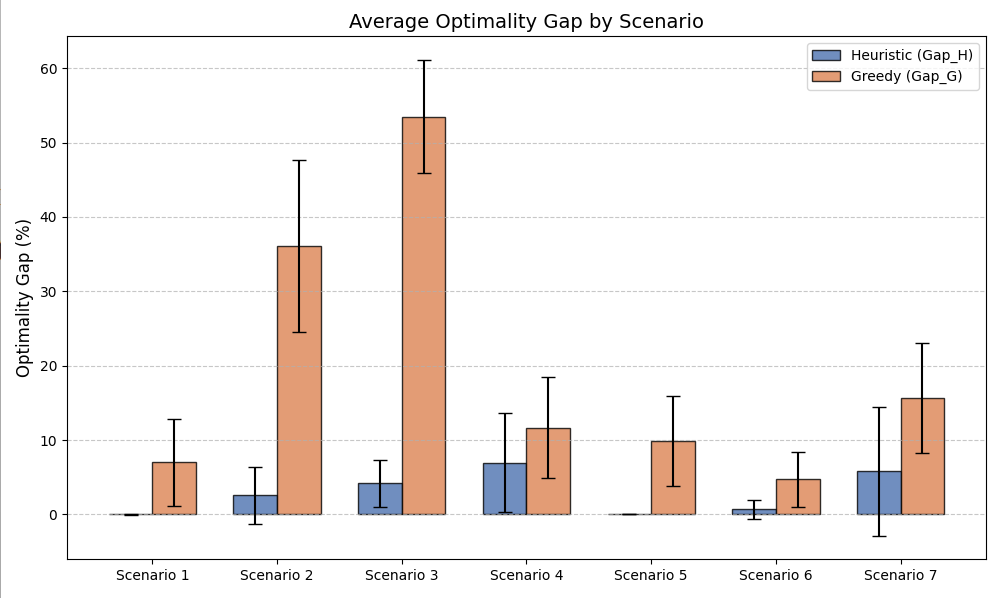
\includegraphics[width=0.95\textwidth]{avg_gap.png}
    \caption{Average Optimality Gap by Scenario}
    \label{fig:performance_chart}
\end{figure}

\end{document}
